\chapter{Workflow di Collaborazione}

\section*{Introduzione}
Un workflow Git definisce come team collabora usando branch, merge e release. Workflow strutturati prevengono caos e garantiscono qualità del codice. Questo capitolo presenta i workflow più popolari: Git Flow, GitHub Flow, Trunk-Based Development, e le pratiche di fork e pull request.

\section*{Obiettivi di apprendimento}
\begin{itemize}
    \item Comprendere perché servono workflow strutturati
    \item Implementare Git Flow per release cicliche
    \item Usare GitHub Flow per deploy continuo
    \item Conoscere Trunk-Based Development
    \item Gestire fork e contribuire a progetti open source
    \item Creare e review Pull Request
    \item Best practices per code review
    \item Strategie di release e versioning
\end{itemize}

\section{Perché Servono Workflow}

\subsection{Il problema senza workflow}

Senza un workflow definito che regoli come il team collabora, il processo di sviluppo diventa rapidamente caotico. Gli sviluppatori cominciano a committare direttamente sul branch main senza coordinamento, causando frequenti rotture in produzione. Feature incomplete finiscono per andare in deploy, rompendo sistemi per gli utenti finali. Quando un problema emerge, è impossibile fare rollback selettivo di una singola feature senza perdere altro lavoro. I bugfix urgenti e le nuove feature diventano mescolati nella storia, rendendo difficile distinguere cosa è stata introdotta quando. I code review, se avvengono, sono inconsistenti e informali. In team con più di due sviluppatori, il risultato è chaos totale: conflitti frequenti, bug introdotti facilmente, e impossibilità di capire chi ha fatto cosa.

\subsection{Workflow risolve}

Un workflow ben definito che standardizza come il team collabora risolve elegantemente questi problemi. Implementa una separazione netta tra feature, hotfix e release, mantenendo isolati i diversi tipi di lavoro. Garantisce che il branch main sia sempre in uno stato deployabile, non contenendo feature incomplete o codice di bassa qualità. Implementa code review obbligatoria attraverso pull request, garantendo che tutto il codice sia revisionato prima di entrare in produzione. Ogni feature ha un branch dedicato, mantenendo tracciabilità chiara di quale lavoro è stato fatto quando. La gestione delle versioni diventa sistematica e ordinata. Infine, grazie alla struttura, è facile tornare indietro se qualcosa va storto, poiché ogni feature è isolata e può essere reverted indipendentemente.

\begin{tcolorbox}[colback=blue!10, colframe=blue!60, title=Scegliere Workflow Giusto]
\textbf{Non esiste workflow perfetto}. Dipende da:
\begin{itemize}
    \item \textbf{Team size}: 2 persone vs 50 persone
    \item \textbf{Release cycle}: Continuous deploy vs release trimestrali
    \item \textbf{Tipo progetto}: Web app vs libreria vs mobile app
    \item \textbf{Cultura team}: Startup agile vs enterprise strutturata
\end{itemize}

Principio guida: \textbf{Semplicità}. Workflow complicato non viene seguito.
\end{tcolorbox}

\section{Git Flow}

\subsection{Panoramica Git Flow}

\textbf{Git Flow} è workflow strutturato creato da Vincent Driessen nel 2010. Ideale per progetti con release cicliche pianificate.

\textbf{Branch principali}:
\begin{description}
    \item[\texttt{main}] Codice in produzione (sempre stabile)
    \item[\texttt{develop}] Branch di integrazione (prossima release)
\end{description}

\textbf{Branch di supporto}:
\begin{description}
    \item[\texttt{feature/*}] Nuove feature (da develop)
    \item[\texttt{release/*}] Preparazione release (da develop)
    \item[\texttt{hotfix/*}] Fix urgenti produzione (da main)
\end{description}

\begin{figure}[h]
    \centering
    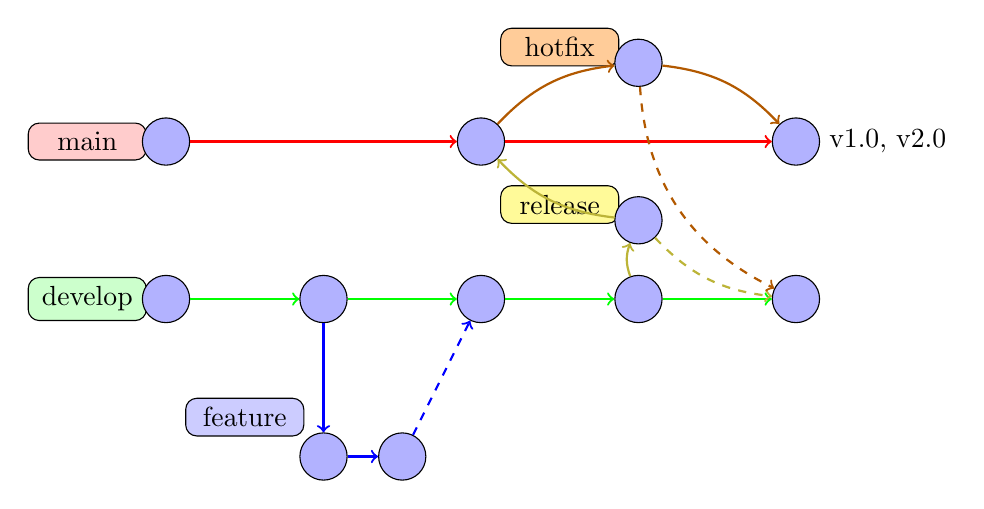
\begin{tikzpicture}[
        commit/.style={circle, draw, fill=blue!30, minimum size=0.6cm},
        branch/.style={rectangle, draw, rounded corners, minimum width=1.5cm},
        arrow/.style={->, thick}
    ]
        % Main branch
        \node[branch, fill=red!20] at (-1, 6) {main};
        \node[commit] (m1) at (0,6) {};
        \node[commit] (m2) at (4,6) {};
        \node[commit] (m3) at (8,6) {};
        \draw[arrow, red, thick] (m1) -- (m2);
        \draw[arrow, red, thick] (m2) -- (m3);
        \node[right] at (8.3,6) {v1.0, v2.0};

        % Develop branch
        \node[branch, fill=green!20] at (-1, 4) {develop};
        \node[commit] (d1) at (0,4) {};
        \node[commit] (d2) at (2,4) {};
        \node[commit] (d3) at (4,4) {};
        \node[commit] (d4) at (6,4) {};
        \node[commit] (d5) at (8,4) {};
        \draw[arrow, green, thick] (d1) -- (d2);
        \draw[arrow, green, thick] (d2) -- (d3);
        \draw[arrow, green, thick] (d3) -- (d4);
        \draw[arrow, green, thick] (d4) -- (d5);

        % Feature branch
        \node[branch, fill=blue!20] at (1, 2.5) {feature};
        \node[commit] (f1) at (2,2) {};
        \node[commit] (f2) at (3,2) {};
        \draw[arrow, blue] (d2) -- (f1);
        \draw[arrow, blue] (f1) -- (f2);
        \draw[arrow, blue, dashed] (f2) -- (d3);

        % Release branch
        \node[branch, fill=yellow!40] at (5, 5.2) {release};
        \node[commit] (r1) at (6,5) {};
        \draw[arrow, yellow!70!black] (d4) to[bend left=20] (r1);
        \draw[arrow, yellow!70!black] (r1) to[bend left=20] (m2);
        \draw[arrow, yellow!70!black, dashed] (r1) to[bend right=20] (d5);

        % Hotfix branch
        \node[branch, fill=orange!40] at (5, 7.2) {hotfix};
        \node[commit] (h1) at (6,7) {};
        \draw[arrow, orange!70!black] (m2) to[bend left=20] (h1);
        \draw[arrow, orange!70!black] (h1) to[bend left=20] (m3);
        \draw[arrow, orange!70!black, dashed] (h1) to[bend right=30] (d5);
    \end{tikzpicture}
    \caption{Git Flow: branch main, develop, feature, release, hotfix}
\end{figure}

\subsection{Feature branches}

\textbf{Scopo}: Sviluppare nuove feature isolate.

\begin{lstlisting}[caption=Workflow feature branch]
# Crea feature branch da develop
$ git checkout develop
$ git checkout -b feature/user-profile

# Sviluppa feature (commit multipli)
$ git add profile.py
$ git commit -m "Add user profile model"
$ git add profile_view.py
$ git commit -m "Add profile view"

# Merge feature in develop (quando completa)
$ git checkout develop
$ git merge --no-ff feature/user-profile
# --no-ff crea merge commit (preserva storia feature)

# Elimina feature branch
$ git branch -d feature/user-profile

# Push develop
$ git push origin develop
\end{lstlisting}

\textbf{Naming convention}:
\begin{itemize}
    \item \texttt{feature/user-authentication}
    \item \texttt{feature/payment-integration}
    \item \texttt{feature/analytics-dashboard}
\end{itemize}

\subsection{Release branches}

\textbf{Scopo}: Preparare nuova release (fix minori, versioning, changelog).

\begin{lstlisting}[caption=Workflow release branch]
# Crea release branch da develop
$ git checkout develop
$ git checkout -b release/1.2.0

# Fix minori, update versioning
$ echo "1.2.0" > VERSION
$ git commit -am "Bump version to 1.2.0"

# Update changelog
$ vim CHANGELOG.md
$ git commit -am "Update changelog for 1.2.0"

# Merge in main (produzione)
$ git checkout main
$ git merge --no-ff release/1.2.0
$ git tag -a v1.2.0 -m "Release version 1.2.0"

# Merge back in develop (per avere fix)
$ git checkout develop
$ git merge --no-ff release/1.2.0

# Elimina release branch
$ git branch -d release/1.2.0

# Push tutto
$ git push origin main develop --tags
\end{lstlisting}

\textbf{Release branch permette}:
\begin{itemize}
    \item Develop continua con nuove feature
    \item Team QA testa release branch
    \item Fix minori su release senza bloccare develop
    \item Deploy quando pronto (non legato a develop)
\end{itemize}

\subsection{Hotfix branches}

\textbf{Scopo}: Fix urgenti in produzione.

\begin{lstlisting}[caption=Workflow hotfix branch]
# Bug critico in produzione (main)
$ git checkout main
$ git checkout -b hotfix/security-patch

# Fix bug
$ vim security.py
$ git commit -am "Fix SQL injection vulnerability"

# Bump version (patch)
$ echo "1.2.1" > VERSION
$ git commit -am "Bump version to 1.2.1"

# Merge in main
$ git checkout main
$ git merge --no-ff hotfix/security-patch
$ git tag -a v1.2.1 -m "Hotfix: security patch"

# Merge in develop (per avere fix)
$ git checkout develop
$ git merge --no-ff hotfix/security-patch

# Elimina hotfix branch
$ git branch -d hotfix/security-patch

# Deploy urgente
$ git push origin main develop --tags
\end{lstlisting}

\subsection{Vantaggi e svantaggi Git Flow}

\begin{tcolorbox}[colback=green!10, colframe=green!60, title=Vantaggi Git Flow]
Git Flow offre una struttura chiara e ben documentata che il team può facilmente seguire e insegnare. È particolarmente adatto per progetti con release pianificate a intervalli regolari (ogni mese, trimestre, ecc.). Il workflow implementa una separazione netta tra il branch di sviluppo (develop) e quello di produzione (main), evitando che feature incomplete compromettano il codice stabile. Gli hotfix per bug critici non bloccano lo sviluppo di nuove feature grazie alla loro separazione. Infine, Git Flow supporta naturalmente il mantenimento di release multiple in parallelo, utile quando è necessario continuare il supporto di versioni precedenti.
\end{tcolorbox}

\begin{tcolorbox}[colback=red!10, colframe=red!60, title=Svantaggi Git Flow]
D'altra parte, Git Flow è eccessivamente complesso per team piccoli o progetti semplici dove questa struttura aggiunge più overhead che valore. La gestione di múltiple branch richiede coordinamento e disciplina costanti. Git Flow non è adatto a continuous deployment o frequent releasing poiché la struttura è pensata per release pianificate. La curva di apprendimento è ripida per sviluppatori junior che devono imparare a navigare tra i diversi branch. Infine, branch longevi (specialmente feature branch) tendono a accumulare merge conflicts frequenti quando il branch di develop avanza mentre il feature branch è ancora in sviluppo.
\end{tcolorbox}

\section{GitHub Flow}

\subsection{Panoramica GitHub Flow}

\textbf{GitHub Flow} è workflow semplificato per continuous deployment. Usato da GitHub stesso e molte startup.

\textbf{Principi}:
\begin{enumerate}
    \item \texttt{main} è sempre deployabile
    \item Feature branch per ogni modifica
    \item Pull request per code review
    \item Deploy dopo merge (continuous)
\end{enumerate}

\textbf{Branch}:
\begin{itemize}
    \item \texttt{main}: Codice in produzione (protetto)
    \item \texttt{feature/*}: Branch temporanei per feature/fix
\end{itemize}

\begin{figure}[h]
    \centering
    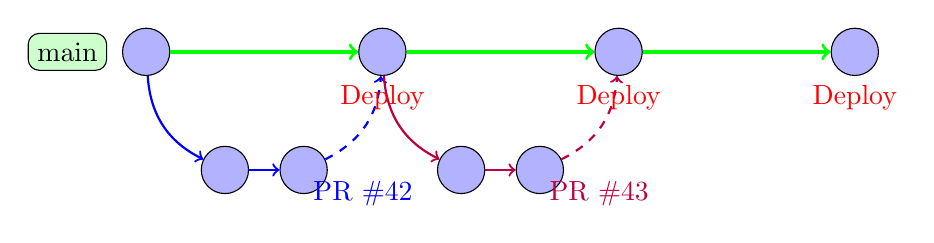
\begin{tikzpicture}[
        commit/.style={circle, draw, fill=blue!30, minimum size=0.6cm},
        branch/.style={rectangle, draw, rounded corners},
        arrow/.style={->, thick}
    ]
        % Main branch
        \node[branch, fill=green!20] at (-1, 3) {main};
        \node[commit] (m1) at (0,3) {};
        \node[commit] (m2) at (3,3) {};
        \node[commit] (m3) at (6,3) {};
        \node[commit] (m4) at (9,3) {};
        \draw[arrow, green, very thick] (m1) -- (m2);
        \draw[arrow, green, very thick] (m2) -- (m3);
        \draw[arrow, green, very thick] (m3) -- (m4);

        % Feature 1
        \node[commit] (f1) at (1,1.5) {};
        \node[commit] (f2) at (2,1.5) {};
        \draw[arrow, blue] (m1) to[bend right=30] (f1);
        \draw[arrow, blue] (f1) -- (f2);
        \draw[arrow, blue, dashed] (f2) to[bend right=30] (m2);
        \node[right, blue] at (2,1.2) {PR \#42};

        % Feature 2
        \node[commit] (f3) at (4,1.5) {};
        \node[commit] (f4) at (5,1.5) {};
        \draw[arrow, purple] (m2) to[bend right=30] (f3);
        \draw[arrow, purple] (f3) -- (f4);
        \draw[arrow, purple, dashed] (f4) to[bend right=30] (m3);
        \node[right, purple] at (5,1.2) {PR \#43};

        % Deploy markers
        \node[below, red] at (3,2.7) {Deploy};
        \node[below, red] at (6,2.7) {Deploy};
        \node[below, red] at (9,2.7) {Deploy};
    \end{tikzpicture}
    \caption{GitHub Flow: main + feature branches + PR + deploy}
\end{figure}

\subsection{Workflow GitHub Flow}

\begin{lstlisting}[caption=GitHub Flow step-by-step]
# 1. Crea feature branch da main
$ git checkout main
$ git pull origin main
$ git checkout -b feature/add-search

# 2. Commit modifiche
$ git add search.py
$ git commit -m "Add basic search functionality"
$ git add search_tests.py
$ git commit -m "Add search tests"

# 3. Push branch
$ git push -u origin feature/add-search

# 4. Apri Pull Request su GitHub
#    - Descrivi modifiche
#    - Request review da colleghi
#    - CI/CD testa automaticamente

# 5. Code review
#    - Colleghi reviewano codice
#    - Suggerimenti e richieste modifiche
#    - Fix e push aggiuntivi

$ git add search.py
$ git commit -m "Address review feedback"
$ git push

# 6. Merge PR (quando approvata)
#    - Merge su GitHub (squash/merge commit/rebase)
#    - CI/CD deploya automaticamente
#    - Branch eliminato automaticamente

# 7. Pull main aggiornato
$ git checkout main
$ git pull origin main
$ git branch -d feature/add-search
\end{lstlisting}

\subsection{Branch protection rules}

\begin{lstlisting}[caption=Proteggere main branch (su GitHub)]
# Settings > Branches > Branch protection rules
# Per "main":
- Require pull request before merging
- Require approvals: 2
- Require status checks to pass (CI)
- Require branches to be up to date
- Require conversation resolution before merging
- Do not allow bypassing the above settings
\end{lstlisting}

\textbf{Effetto}:
\begin{itemize}
    \item Impossibile push diretto a \texttt{main}
    \item Tutte le modifiche via Pull Request
    \item Review obbligatoria (2 approvazioni)
    \item Test devono passare
    \item Garantisce qualità codice
\end{itemize}

\subsection{Vantaggi e svantaggi GitHub Flow}

\begin{tcolorbox}[colback=green!10, colframe=green!60, title=Vantaggi GitHub Flow]
GitHub Flow è notevolmente semplice: usa solo un branch principale con feature branch temporanei, eliminando la complessità di múltiple branch di integrazione. È ideale per continuous deployment e release frequenti poiché la struttura è pensata per deploy veloci e ripetuti. Il code review è integrato naturalmente attraverso pull request, rendendo facile la revisione del codice prima del merge. I deploy frequenti (anche diverse volte al giorno) mantengono le feature in produzione rapidamente. I branch sono short-lived (di breve durata), riducendo la probabilità di merge conflicts. La curva di apprendimento è bassa: gli sviluppatori hanno solo bisogno di imparare a creare feature branch e fare pull request.
\end{tcolorbox}

\begin{tcolorbox}[colback=red!10, colframe=red!60, title=Svantaggi GitHub Flow]
GitHub Flow non è adatto a progetti con release pianificate perché manca la struttura per gestire versioni parallele. Richiede un CI/CD robusto e affidabile per funzionare correttamente, poiché ogni merge in main viene deployato. Richiede anche testing automatico esteso per compensare l'assenza di un branch di integrazione dedicato. È difficile gestire múltiple versioni in produzione contemporaneamente. Infine, gli hotfix per bug critici sono trattati come feature branch normali, senza prioritization speciale.
\end{tcolorbox}

\section{Trunk-Based Development}

\subsection{Panoramica}

\textbf{Trunk-Based Development} è workflow estremo: sviluppatori committano direttamente su \texttt{main} (trunk) o usano branch brevissimi (1-2 giorni max).

\textbf{Principi}:
\begin{itemize}
    \item Un branch principale (\texttt{main}/\texttt{trunk})
    \item Commit piccoli e frequenti
    \item Feature flags per feature incomplete
    \item CI/CD estremamente robusto
    \item Test automatici estesi
\end{itemize}

\begin{lstlisting}[caption=Trunk-Based Development]
# Commit diretto su main (se feature completa)
$ git checkout main
$ git pull
$ git add feature.py
$ git commit -m "Add small feature (behind feature flag)"
$ git push

# Oppure branch brevissimo (max 1-2 giorni)
$ git checkout -b quick-fix
$ git commit -am "Fix navbar alignment"
$ git push -u origin quick-fix
# Immediate PR + merge (stesso giorno)
\end{lstlisting}

\subsection{Feature flags}

\begin{lstlisting}[caption=Feature flags per trunk-based]
# Codice in produzione ma feature disabilitata
def new_dashboard():
    if feature_flag('new_dashboard_enabled'):
        return render_new_dashboard()
    else:
        return render_old_dashboard()

# Deploy codice incomplete ma safe
# Abilita feature quando pronta (runtime toggle)
\end{lstlisting}

\textbf{Vantaggi}:
\begin{itemize}
    \item Deploy continuo anche con feature incomplete
    \item Test in produzione con subset utenti
    \item Rollback istantaneo (toggle flag)
    \item No branch longevi
\end{itemize}

\subsection{Quando usare Trunk-Based}

Trunk-Based Development è adatto per team senior esperti con una culture DevOps forte e un CI/CD maturo e affidabile. Richiede che il test coverage sia superiore al 90% per garantire che il codice deployato sia stabile. Questo workflow è ideale per ambienti che richiedono deploy multipli al giorno.

Al contrario, non è adatto per team junior che potrebbero non avere la disciplina necessaria per fare commit piccoli e frequenti su main. Non funziona per progetti senza infrastruttura CI/CD solida. Se il team richiede code review formale e strutturata, questa non è la scelta giusta. Infine, non è adatto per progetti con release pianificate che seguono un ciclo di versioning tradizionale.

\section{Pull Request e Code Review}

\subsection{Cos'è una Pull Request}

\textbf{Pull Request (PR)} è richiesta di merge branch feature in branch principale. Include:
\begin{itemize}
    \item Descrizione modifiche
    \item Diff completo del codice
    \item Conversazione/commenti
    \item Review/approvazioni
    \item Status check CI/CD
\end{itemize}

\subsection{Creare Pull Request efficace}

\begin{tcolorbox}[colback=green!10, colframe=green!60, title=Template Pull Request]
\textbf{Titolo}: Add user authentication with JWT

\textbf{Description}:
\begin{verbatim}
## Cosa cambia
- Implementa JWT authentication
- Aggiunge login/logout endpoints
- Protegge API endpoints

## Perché
Richiesto per proteggere API da accessi non autorizzati.

## Come testare
1. POST /api/login con username/password
2. Ricevi JWT token
3. Usa token in header Authorization: Bearer <token>
4. Accedi a /api/protected (prima restituiva 401)

## Checklist
- [x] Test scritti e passano
- [x] Documentazione aggiornata
- [x] Nessun breaking change
- [x] Code review requested

## Screenshots
[Allegati screenshot se UI changes]

Fixes #123
\end{verbatim}
\end{tcolorbox}

\subsection{Code Review Best Practices}

Per chi scrive una pull request, è importante mantenerla piccola: idealmente meno di 200 righe, comunque non più di 400. Una descrizione chiara e completa del cambiamento è essenziale. Prima di richiedere revisione, dovresti fare una self-review per catturare errori evidenti. I test inclusi nella PR devono passare. Ogni PR dovrebbe rappresentare una singola feature o fix, non una miscellanea di cambiamenti. Quando ricevi feedback, rispondi costruttivamente e non prendere i commenti come critica personale.

Per chi reviziona, è importante fornire feedback entro 24 ore per non bloccare il lavoro di altri. Il feedback dovrebbe essere costruttivo e non una critica personale dello scrittore. Distingui chiaramente tra "must fix" (problemi bloccanti) e "nice to have" (miglioramenti suggeriti). Approva il PR quando è "abbastanza buono" - la perfezione è nemica del bene. Se trovi molti commenti da fare, considera di fare una call sincrona con l'autore invece di intavolare 50 commenti scritti.

\begin{lstlisting}[caption=Commenti review esempi]
# Bad review comment
"This is wrong."

# Good review comment
"Considera usare dict comprehension qui per migliore readability:
users = {u.id: u for u in user_list}
Cosa ne pensi?"

# Nitpick (non blocking)
"Nit: Typo in commento 'recieve' -> 'receive'"

# Blocking (must fix)
"Questo causa SQL injection. Usa parametrized query:
cursor.execute('SELECT * FROM users WHERE id = ?', (user_id,))"
\end{lstlisting}

\subsection{Merge strategies su PR}

\textbf{Merge commit} (default):
\begin{itemize}
    \item Preserva storia completa
    \item Crea merge commit
    \item Storia non lineare
\end{itemize}

\textbf{Squash and merge}:
\begin{itemize}
    \item Tutti commit feature → 1 commit
    \item Storia main pulita
    \item Perde storia intermedia feature
\end{itemize}

\textbf{Rebase and merge}:
\begin{itemize}
    \item Replay commit su main
    \item Storia lineare
    \item Nessun merge commit
\end{itemize}

\begin{lstlisting}[caption=Configurare merge strategy (GitHub)]
# Settings > General > Pull Requests
- Allow merge commits
- Allow squash merging (raccomandato per feature)
- Allow rebase merging

# Default: squash per main, merge per develop
\end{lstlisting}

\section{Confronto Workflow}

\begin{table}[h]
\centering
\begin{tabular}{|l|c|c|c|}
\hline
\textbf{Caratteristica} & \textbf{Git Flow} & \textbf{GitHub Flow} & \textbf{Trunk-Based} \\
\hline
Complessità & Alta & Bassa & Molto bassa \\
Branch principali & 2 (main+develop) & 1 (main) & 1 (main) \\
Branch supporto & 3 tipi & 1 tipo & Nessuno/brevi \\
Release cycle & Pianificato & Continuo & Continuo \\
Team size & Grande & Medio & Piccolo/senior \\
CI/CD & Consigliato & Richiesto & Essenziale \\
Code review & Opzionale & Obbligatorio & Opzionale \\
Curva apprendimento & Ripida & Moderata & Bassa \\
\hline
\end{tabular}
\caption{Confronto workflow Git}
\end{table}

\section*{Riepilogo concetti chiave}

\begin{tcolorbox}[colback=gray!10, colframe=black!60, title=Concetti fondamentali]
\begin{itemize}
    \item \textbf{Workflow} definisce come team collabora con Git
    \item \textbf{Git Flow}: main+develop, feature/release/hotfix, release pianificate
    \item \textbf{GitHub Flow}: main+feature, PR, continuous deployment
    \item \textbf{Trunk-Based}: commit diretti/branch brevissimi, feature flags
    \item \textbf{Pull Request}: Richiesta merge + code review + CI
    \item \textbf{Branch protection}: Impedisce push diretto, forza PR
    \item \textbf{Code review}: Qualità codice, knowledge sharing
    \item \textbf{Merge strategies}: merge commit vs squash vs rebase
    \item Workflow dipende da: team size, release cycle, CI/CD maturity
    \item \textbf{Semplicità} è chiave: workflow complesso non viene seguito
\end{itemize}
\end{tcolorbox}

\section*{Esercizi}

\begin{enumerate}
    \item Simula Git Flow: crea \texttt{develop}, feature branch, release branch, merge in \texttt{main}.

    \item Pratica GitHub Flow: crea feature, push, apri PR (su GitHub), merge.

    \item Configura branch protection su repository GitHub per \texttt{main}.

    \item Scrivi PR description completa per feature recente (usa template).

    \item Fai code review di PR (proprio o altrui), pratica commenti costruttivi.

    \item Sperimenta merge strategies: merge commit vs squash vs rebase, confronta storia.

    \item Simula hotfix workflow in Git Flow.

    \item Configura GitHub Actions per CI su PR (test automatici).

    \item Crea fork, contribuisci a progetto open source, apri PR.

    \item Discuti con team quale workflow è adatto al vostro progetto.
\end{enumerate}

\section*{Riferimenti}

\begin{itemize}
    \item Git Flow originale: \url{https://nvie.com/posts/a-successful-git-branching-model/}
    \item GitHub Flow: \url{https://guides.github.com/introduction/flow/}
    \item Trunk-Based Development: \url{https://trunkbaseddevelopment.com/}
    \item Code Review Best Practices: \url{https://google.github.io/eng-practices/review/}
    \item Pull Request template: \url{https://docs.github.com/en/communities/using-templates-to-encourage-useful-issues-and-pull-requests}
\end{itemize}
